
\documentclass[12pt,a4paper]{article}

\usepackage{rotating}
\usepackage{fancyhdr}
\usepackage{url}
\usepackage{hyperref}
\usepackage{amsmath}
\usepackage{amssymb}
\usepackage{bm}
\usepackage{soul}
\usepackage{graphicx}
\usepackage[cm]{fullpage}
\usepackage{float}
\usepackage{color,soul,xcolor,colortbl}
\usepackage{framed}


%\floatstyle{boxed} 
%\restylefloat{figure}


% \renewcommand{\labelitemi}{$\bullet$}
% \renewcommand{\labelitemi}{$\circ$}
\renewcommand{\labelitemii}{$\circ$}
% \renewcommand{\labelitemii}{$\cdot$}
% \renewcommand{\labelitemiii}{$\diamond$}
% \renewcommand{\labelitemiv}{$\ast$}

\pagestyle{fancy}
\renewcommand{\headrulewidth}{0pt}
\renewcommand{\footrulewidth}{0.3pt}
\fancyhf{}
\lfoot{\footnotesize{Copyright \copyright  \space   \the\year \space The University of Technology Sydney (UTS), Australia.}}
\rfoot{\small{page \thepage}}


\begin{document}


\sethlcolor{yellow}

\pdfpkresolution=2400
\pdfcompresslevel=0
\pdfobjcompresslevel=0
\pdfdecimaldigits=9


\setlength{\parindent}{0pt}
\setlength{\parskip}{2ex}


\begin{titlepage}
\begin{center}


% Title

\vspace*{3cm}

\rule{\linewidth}{0.5mm} \\[0.4cm]
{ \huge \bfseries GMNL2a }\\[0.4cm]
{\large \textsc{GMNL-II with additive approximated afterthought}}

{\large \emph{A maximum likelihood model -- a GMNL-II variation on the ``scale vs. preference'' theme.}}
\rule{\linewidth}{0.5mm}
\\[1.1cm]
\large
\textit{Leon(id) Zadorin}
\vspace{3cm}

{\Large \textsc{Centre for the Study of Choice (CenSoC)}}

{\large University of Technology Sydney (UTS), Australia.}


\vfill

\emph{Built from \LaTeX.} \\ 
\InputIfFileExists{git_hash.txt}{\emph{Git-repository contents revision:} \\}{\hl{UNVERSIONED build}}
% {\small \input{git_hash.txt}}

% Bottom of the page
Copyright \copyright  \space   \the\year \space The University of Technology Sydney (UTS), Australia.

\end{center}

\end{titlepage}

\newpage
\tableofcontents
\newpage
\section{Introduction}

At present, this document should invariably be considered a ``work-in-progress'' -- to the point of representing a ``thinking out loud'' process where some things could well be very wrong, or they could be quite correct; the contents could make absolutely no sense or they could lead to a useful model.

Moreover, given that I (Leon) am not a qualified scientist/academic/researcher in the area of mathematics, statistics, probability and choice modeling -- but rather a software (IT) architect, analyst and developer -- any of the content with respect to the theoretical/model propositions and analysis should not be seen as being necessarily-endorsed by (or spoken on behalf of) the university. 

In other words -- ``take it with a grain of salt''.

The document exists for the purposes of transparency and account-keeping so to speak -- it some thoughts and variations on the theme of Generalized Multinomial Logit (GMNL) and, specifically, part thereof: the GMNL-II. 

Such variations are conducted in light of attempting to better assimilate any of the numerically-scaled relationships amongst respondents' preferences.

The issues relating to possible misinterpretation of the numerically-scaled relationship for other, non preference-homogeneous, factors are deemed to be outside the scope of this document (and shall, perhaps, be happily addressed later on -- in other ramblings). 

Consequently, as far as this document is concerned -- ``if it looks like a scale then it is a scale'' (i.e. a set of homogeneous preferences).

Moreover, the following choice-characterization of the underlying respondents' data is not aimed at being identified by Gmnl2a:
\begin{itemize}
\item ``Distance from zero'' -- the model essentially discards any semantics associated with how close-to (or far from) zero-line a given respondent's beta values happen to be. There is no preservation of how confident or unsure a given respondent's preference happens to be.
\item ``Proportional inter-attribute relationships'' -- the model does not attempt to preserve/identify the ratio(s) between various attributes. Consequently, those surveys which aim at dealing with such ratios (e.g. willingness to pay) may need to understand this point rather well. 
\end{itemize}

The model (Gmnl2a) only concerns itself with a differential relationship between attributes (such may be normalized/scaled to a given boundary for the purpose of juxtaposition with other models' results, but the notion of differential relationship stands) -- that is to say: ``how much one attribute is more/less important in comparison to another, where importance is essentially a distance between the attributes' beta values''.

\section{Background}

Given the following characterization of GMNL-II:
{ \Large 
\begin{equation}
\label{eq:gmnl_2a_1}
U=\sigma(\pmb{\hm{\beta}}+\pmb{\hm{\eta}}) + \varepsilon
\end{equation}
}

one may see GMNL-II as a rather intuitive mechanism for dealing with a numerically-scaled relationship amongst preferences recorded in the underlying dataset (i.e. the semantic preferences of various respondents present in the completed survey's data). Scaled relationship, that is, which was caused by a respondent-specific variation in the amplitude of  \(\varepsilon\) -- user's ``sensitivity to the unobserved attributes'' in laymen terms.

The simplification process, when evaluating GMNL-II, may well be extended to a point where one is essentially interested in identifying \textit{only} the \(\hm{\beta}\) and \(\hm{\eta}\). 

The scale distribution \(\sigma\) itself is, arguably, not so important in it's explicit characterization -- any  account for ``de-scaling'' benefits achieved by GMNL-II could be inferred from a direct comparison of  \(\hm{\eta}\) with that of a traditional mixed logit: \(U=\hm{\beta}+\hm{\eta} + \varepsilon\) where, without the ``scale-absorbing'' \(\sigma\), any of the ``numerically-proportional'' relationships between preferences would be usurped by (or rather attributed to) the increase in \(\hm{\eta}\) as illustrated in figure~\ref{fig:variances_compared_1} p.\pageref{fig:variances_compared_1}.


\begin{sidewaysfigure}
% \begin{figure}[H]
\begin{framed}
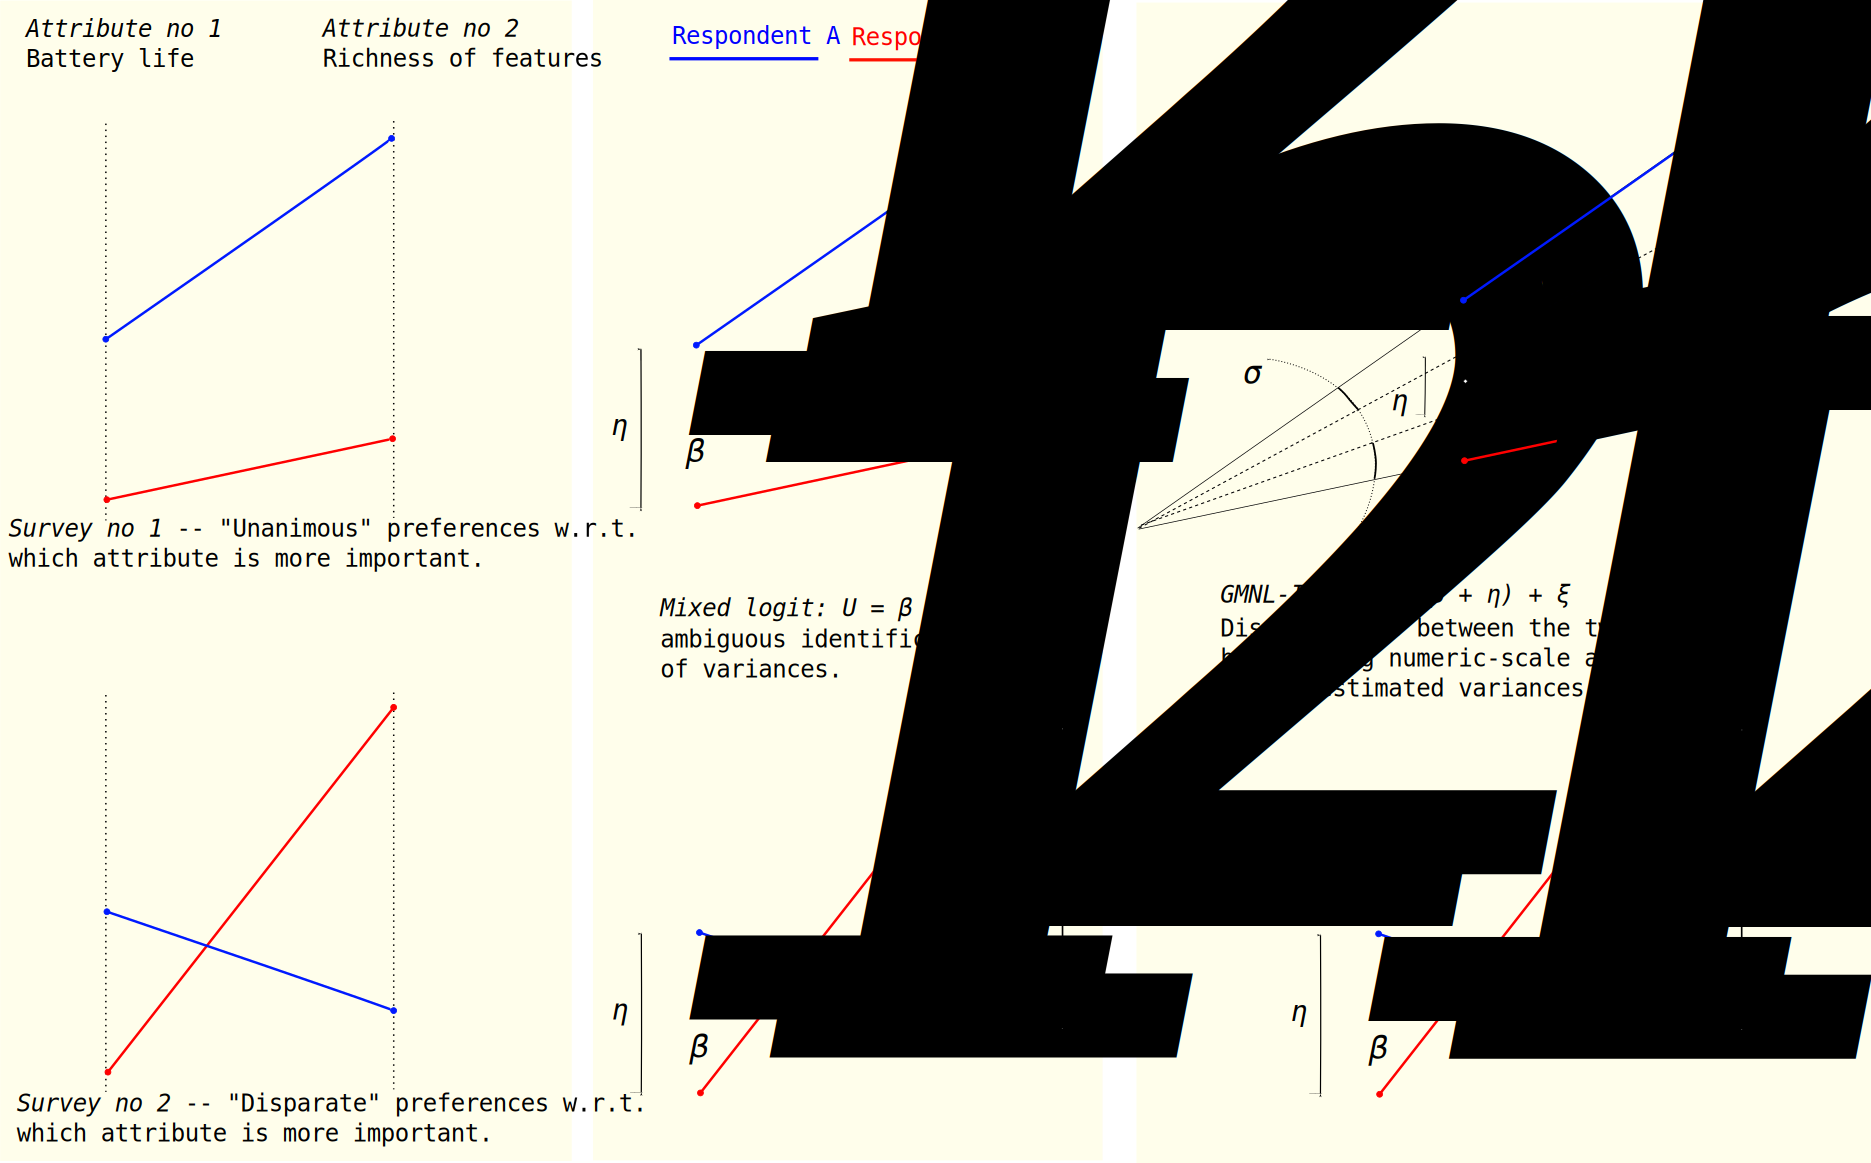
\includegraphics[width=\textwidth, keepaspectratio = true]{pics/intuitive_proposition_1.eps}

Depicts two fictitious surveys for the mobile phones where preferences for the battery-life vs the richness-of-features are considered. Presume that each of the respondents has enough observations to have basic logit evaluated individually per respondent.

\caption{Mixed logit vs GMNL-II and relevant (in)ability to separate scale from variance.} 

\label{fig:variances_compared_1}
\end{framed}
% \end{figure}
\end{sidewaysfigure}

\newpage
Before proceeding any further, it would behoove one to consider how models such as GMNL, mixed logit, et al. actually calculate/determine their parameters during convergence.

The arithmetic of the models appears to be such that it picks only \textit{one} \(\pmb{\hm{\beta}}\) vector as a solution and then, by virtue of some transformation formula, produces a whole \textit{set of transformed beta vectors}. Such a set is then ``tested'' for the likelihood it produces w.r.t. to various respondents' data (i.e. how well all of such transformed beta vectors ``fit'' the data). 

The aforementioned process is usually done many times (each time with a differently picked solution, but with common mechanisms of transformation) and the set yielding the highest likelihood denotes the converged-on parameters for the model. The parameters would include a single vector of betas \(\pmb{\hm{\beta}}\) used to produce the winning set and any other transformation-describing parameters (e.g. variances \(\pmb{\hm{\eta}}\) of the distributions used in the ``transformation'' process).

As an example, consider basic/traditional mixed logit model: \(U=\hm{\beta}+\hm{\eta} + \varepsilon\) (let us suppose that only the uncorrelated normal distributions for \(\pmb{\hm{\eta}}\)  are used in such a model).

The convergence process would essentially start by choosing candidate vectors \(\pmb{\hm{\beta}}\) and \(\pmb{\hm{\eta}}\). Next, for each element of \(\pmb{\hm{\beta}}\), a draw from a normal distribution (with variance of \(\pmb{\hm{\eta}}\)) will be made and added to the relevant member of \(\pmb{\hm{\beta}}\) resulting in a single instance of the transformed candidate vector. 

In order to generate a whole set of such vectors, the transformation process is repeated many times where candidate vectors do not change (but the values produced by the draws from the distribution obviously vary -- the distribution draws themselves may be done at random or with the help of Halton sequences, etc. but this is largely irrelevant here).

The whole of the resulting set is then tested for the produced likelihood with respect to the underlying survey data.

The key factor in the above descriptions is that only \textit{one} vector of betas (\(\pmb{\hm{\beta}}\)) is picked as the input to the transformation process in order to yield a \textit{set} of transformed betas.

The critical characterization then becomes for the \textit{transformation} process (i.e. a \textit{holistic} mechanism of transformation applied \textit{consistently} to one, single \(\pmb{\hm{\beta}}\)) to produce the best-possible, most-harmonious set of \(\pmb{\hm{\beta}}\)s which would ``fit'' the underlying data (e.g. individual respondents' beta vectors) as much as possible.

Whilst figure~\ref{fig:variances_compared_1} p.\pageref{fig:variances_compared_1} appears to show no concern for such a requirement for GMNL-II (as it's scaling transformation covers the underlying preferences reasonably well) the issue becomes more critical if/when \textit{negative} beta values are present in the semantically underlying respondents' preferences (see figure~\ref{fig:negative_betas_1} p.\pageref{fig:negative_betas_1}). \hl{TODO -- verify that it is indeed infeasible to generate survey datasets where the resulting respondents' betas are all non-negative in the first place...}


\begin{figure}[H]
\begin{framed}
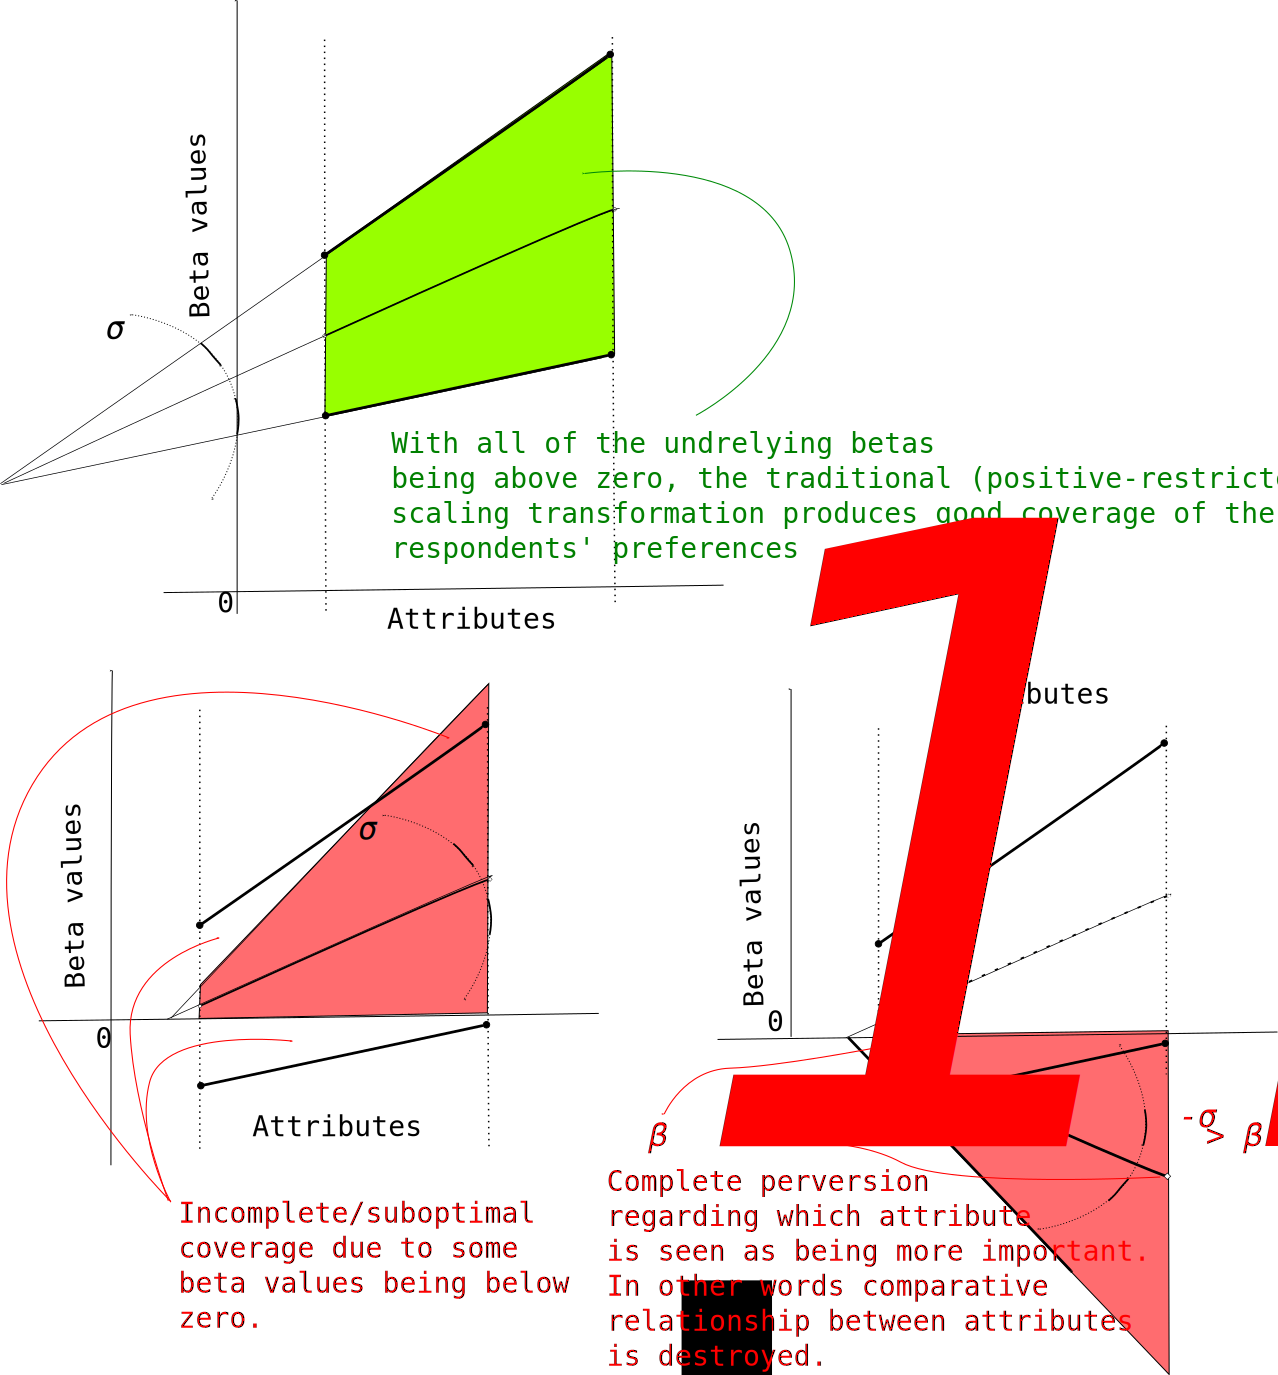
\includegraphics[width=\textwidth, keepaspectratio = true]{pics/negative_betas_1.eps}


\caption{Issues associated with the scaling transformation when some of the underlying betas are negative.} 

\label{fig:negative_betas_1}
\end{framed}
\end{figure}

It might be of interest to momentarily digress and note that mixed logit model is not affected by such a scenario (i.e. it is able to ``fit'' the data equally well irrespective of whether some semantically underlying betas are negative) -- because it's transformation process yields an offsetting/additive process (i.e. distribution draws are \textit{added} to \(\pmb{\hm{\beta}}\)). This points to an auxiliary notion that some transformations are more sensitive to positioning of the underlying betas than others.


\section{GMNL2a}

Given that scaling transformation is at the very center of GMNL-II, one is simply unable to ignore the aforementioned ``negative betas'' difficulties. To such an extent, it is possible to propose a cumulative/holistic offset for the transformational post-processing. 

In other words, the finally-produced set of scale-distributed betas is further transposed up and down before being tested for how well it fits the underlying dataset. 

Alternatively, one may visualize a semantically-equivalent process of applying a GMNL-II model to the transposed/shifted set of the underlying respondents' preferences/betas  (i.e. transformed dataset). Figure figure~\ref{fig:gmnl2a_offsetting_1} p.\pageref{fig:gmnl2a_offsetting_1} attempts to illustrate such a visualization.

\begin{figure}[H]
\begin{framed}
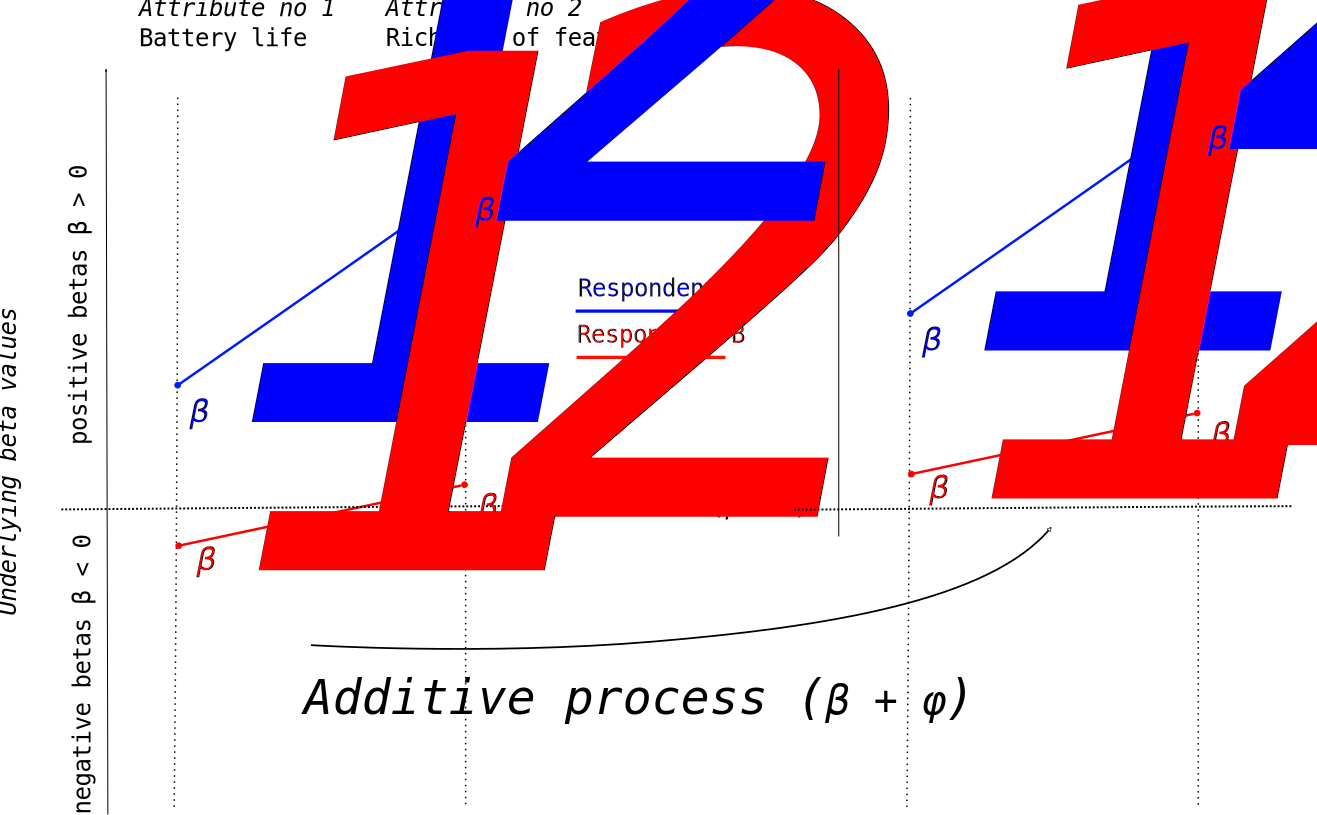
\includegraphics[width=\textwidth, keepaspectratio = true]{pics/gmnl2a_offsetting_1.eps}
\caption{\textit{Additive} post-processing as a part of the transformation process.} 
\label{fig:gmnl2a_offsetting_1}
\end{framed}
\end{figure}

\subsection{Additive}

The GMNL2a then becomes:
{ \Large 
\begin{equation}
\label{eq:gmnl_2a_1}
U=\phi + \sigma(\pmb{\hm{\beta}}+\pmb{\hm{\eta}}) + \varepsilon
\end{equation}
}

where the additional scalar \(\phi\) is introduced -- representing an overall additive/subtractive offset for the produced set of transformed betas. 

\subsection{Approximation}

Undoubtedly, however, the offsetting process happens to be an approximation -- the act of moving a whole set of beta vectors up/down in their absolute values is going to compromise any of the existing scale relationships (and possibly introduce some new ones).

For example, given numeric scale between respondents' preferences in the \textit{original} dataset (as illustrated by equation ~\ref{eq:gmnl_2a_2} p.\pageref{eq:gmnl_2a_2} -- with superscripts denoting respondents and subscripts indicating attributes):

{ \Large 
\begin{equation}
\label{eq:gmnl_2a_2}
\frac{\beta^{^1}_{1}}{\beta^{^2}_{1}}=\frac{\beta^{^1}_{2}}{\beta^{^2}_{2}}
\end{equation}
}

the act of adding a constant to each of the betas may no longer yield the aforementioned (eq. ~\ref{eq:gmnl_2a_2} p.\pageref{eq:gmnl_2a_2}) equivalence as per equation ~\ref{eq:gmnl_2a_3} p.\pageref{eq:gmnl_2a_3}:

{ \Large 
\begin{equation}
\label{eq:gmnl_2a_3}
\frac{\beta^{^1}_{1} + \phi}{\beta^{^2}_{1} + \phi} \neq \frac{\beta^{^1}_{2} + \phi}{\beta^{^2}_{2} + \phi}
\end{equation}
}

To such an extent, the offset could cause a lesser perception of scale (i.e. smaller distribution of \(\sigma\)) at the invariable expense of, now incorrectly determined, higher variance values \(\pmb{\hm{\eta}}\).

Such a compromise, however, is not expected to be of significant detriment. Indeed, the value of \(\vert \phi \vert\) could be used as a potential indicator as to the extent of possible misinterpretation and is not expected to be particularly large in a multitude of practically-feasibly scenarios.

\subsection{Afterthought}

With respect to the GMNL model, and it's underlying theoretical foundations, \(\phi\) is really an afterthought -- in that it does not feature explicitly at the theoretical level, but rather at the stage of numeric ``fitting'' considerations/challenges when converging on the aggregated set of multiple respondents' preferences.

\subsection{Post-convergence normalization}

After the convergence is completed there is a need to counter any of the offsets/``distortions'' produced by the aforementioned modulation. Cumulatively speaking, a certain process is applied in order to produce parameters (\(\pmb{\hm{\beta}}\) and \(\pmb{\hm{\eta}}\)) to be of comparable values when juxtaposed with other, similar to GMNL2a, models (e.g. GMNL-I, GMNL-II, mixed logit and so on):

\begin{itemize}

\item \(\sigma\) is discarded (as per the aforementioned GMNL-II simplification notion)

\item \( \phi \) is subtracted from \( \pmb{\hm{\beta}} \)

\item the resulting \( \pmb{\hm{\beta}} \) and \( \pmb{\hm{\eta}} \) are normalized -- each element of the aforementioned vector is scaled by a constant. The constant value is determined in such a way that the normalization process makes the absolute value of the largest \( \pmb{\hm{\beta}} \) element equal to \(1\). Such a normalization process is envisaged to be applied to other, comparable, models (e.g. \( \pmb{\hm{\beta}} \) and \( \pmb{\hm{\eta}} \) in mixed logit). This allows for cross-model comparison with respect to the obtained attribute-preferences within a group of respondents and their respective heterogeneity of the opinion (i.e. variances).
\end{itemize}

For example, given the following ``raw'' estimated parameters:

\begin{itemize}
\item \( \phi = 3 \)
\item \(\pmb{\hm{\beta}} = \{2, 1, 3, 5\}\)
\item \(\pmb{\hm{\eta}} = \{0.5, 3, 2, 0.1\}\)
\end{itemize}

the ``massaged'' output would be generated in the following manner:

\begin{itemize}
\item Offset the beta values, \(\pmb{\hm{\beta}} = \{2-3, 1-3, 3-3, 5-3\} = \{-1, -2, 0, 2\}\)
\item Obtain normalization constant \(=2\)
\item Scale both the \( \pmb{\hm{\beta}} \) and \( \pmb{\hm{\eta}} \) by \(\frac{1}{2}\)
\item \(\pmb{\hm{\beta}} = \{-0.5, -1, 0, 1\}\)
\item \(\pmb{\hm{\eta}} = \{0.25, 1.5, 1, 0.05\}\)
\end{itemize}

In a similar fashion, if a different model (e.g. mixed logit) had converged on the same dataset with the following ``raw'' parameters:

\begin{itemize}
\item \(\pmb{\hm{\beta}} = \{-1.5, -3, 0, 3\}\)
\item \(\pmb{\hm{\eta}} = \{1, 6, 4.5, 1.5\}\)
\end{itemize}

Then it's normalization process would yield:
\begin{itemize}
\item Obtain normalization constant from betas \(=3\)
\item Scale both the \( \pmb{\hm{\beta}} \) and \( \pmb{\hm{\eta}} \) by \(\frac{1}{3}\)
\item \(\pmb{\hm{\beta}} = \{-0.5, -1, 0, 1\}\)
\item \(\pmb{\hm{\eta}} = \{0.33, 2, 1.5, 0.5\}\)
\end{itemize}

Finally two models would be juxtaposed with respect to their parameters (e.g. \(\pmb{\hm{\eta}}\) values). Naturally, the aforementioned example illustrates \(\pmb{\hm{\beta}}\)'s absolute equality rather naively, but the thesis of the intent for the post-normalization process remains. 

\subsection{Further models -- SOMML (Scaled Offset Mixed Multinomial Logit)}

Given that the model in question (i.e. Gmnl2a) only attempts to identify \textit{differential} relationships between attributes, one may consider ``\textit{parallel}'' betas (i.e. no scale, just the offset) from \textit{different} respondents as also being synonymous. For example, in a case of two respondents and two attributes, the following data could be considered synonymous: \(\{\beta^{^1}_{1} = 1, \beta^{^1}_{2} = 2\} == \{\beta^{^2}_{1} = -2, \beta^{^2}_{2} = -1\}\) because  \(\beta^{^1}_{2} - \beta^{^1}_{1}  = \beta^{^2}_{2} - \beta^{^2}_{1} = 1\)

To account for such a ``parallelism'', one may introduce additional \textit{offsetting distribution} prior to scaling:
{ \Large 
\begin{equation}
\label{eq:somml_1}
U=\phi + \sigma(\Phi + \pmb{\hm{\beta}}+\pmb{\hm{\eta}}) + \varepsilon
\end{equation}
}

where \(\Phi\) is not a scalar, constant across different respondents; but rather, in a fashion similar to \(\sigma\), is re-drawn for each of the respondents from an arbitrary (e.g. normal) distribution.

Such a process is left for further experimentation (even though the SOMML code has, practically, been written alredy) -- as it shall invariably introduce additional computational requirements:
\begin{itemize}
\item estimation of the mean of \(\Phi\)
\item estimation of the variance of \(\Phi\) -- a process which involves redrawing a set of values and recalculating \textit{vector}-based arithmetic (i.e. not just a coefficient's value being injected in a simple sum, but rather a ``number of draws'' repetitive computations).
\end{itemize}

Even though such computations may not be used in the final solution (e.g. variance of \(\Phi\) may be discarded in a fashion similar to that of \(\sigma\)'s influence on the finally-presented set of coefficients), the computations will still need to be conducted during the convergence process.

Given that, generally, distribution-based identification (e.g. \(\sigma\), etc.) is not 100\% precise anyway (i.e. who can possibly expect any given fixed-shape distribution to completely fit a realistic case), and that the aforementioned cases of ``offsetting'' approximation are not anticipated to drastically corrupt ``scale relationships'' (and vice versa) -- the identification benefits of \(\Phi\) need to be empirically tested for in order to determine whether they are worthy of the inevitable slowdown in computation/performance... anyway a \hl{TODO} for the future musings when the time allows :-) :-) :-) ... 

\end{document}
